% Apêndice B: arquivo binário com registros de tamanho fixo (40 bytes) e um índice em memória.
\documentclass[border=4pt]{standalone}
\usepackage[utf8]{inputenc}
\usepackage[T1]{fontenc}
% Estilo comum das figuras de vetores (capítulo 8).
\usepackage{tikz}
\usetikzlibrary{arrows.meta, positioning, calc, decorations.pathreplacing}
\definecolor{navy}{RGB}{23,45,80}
\definecolor{laranja}{RGB}{250,110,29}
\definecolor{cinzalogo}{RGB}{107,114,126}
\definecolor{azul}{RGB}{205,222,247}
\tikzset{
  casa/.style={draw=navy, line width=0.9pt, minimum width=8mm, minimum height=7mm,
               inner sep=0pt, font=\sffamily\small},
  pronta/.style={casa, fill=azul},
  parte/.style={casa, fill=laranja!12},
  marcada/.style={casa, fill=laranja!45, draw=laranja},
  fora/.style={casa, draw=cinzalogo!60, dashed, fill=white, text=cinzalogo!60},
  indice/.style={font=\sffamily\scriptsize, text=cinzalogo},
  explica/.style={font=\sffamily\small, text=navy, anchor=east},
  legenda/.style={font=\sffamily\scriptsize, text=cinzalogo},
  rotulo/.style={font=\sffamily\small\bfseries, text=navy},
  seta/.style={-{Stealth[length=2.2mm]}, navy, line width=0.9pt},
  chave/.style={decorate, decoration={brace, amplitude=4pt, mirror}, navy, line width=0.8pt},
}
% \vetor{nome}{x}{y}{valor/estilo, valor/estilo, ...}: casas lado a lado, chamadas nome0, nome1...
\newcommand{\vetor}[4]{%
  \foreach \valor/\estilo [count=\i from 0] in {#4} {
    \node[\estilo] (#1\i) at ($(#2, #3) + (\i*0.8, 0)$) {\valor};
  }
}

\tikzset{
  campo/.style={draw=navy, line width=0.8pt, minimum height=8mm, inner sep=1pt,
                font=\sffamily\scriptsize, align=center},
  byte/.style={font=\sffamily\scriptsize, text=cinzalogo},
  chaveidx/.style={draw=navy, line width=0.8pt, minimum width=14mm, minimum height=6mm,
                   font=\sffamily\scriptsize, fill=azul},
}
% \registro{nome}{x}{matrícula}{nome do aluno}{nota}: 4 + 24 (+4 de preenchimento) + 8 bytes
\newcommand{\registro}[5]{%
  \node[campo, fill=laranja!12, minimum width=7mm, anchor=west] (#1m) at (#2, 0) {#3};
  \node[campo, fill=white, minimum width=17mm, anchor=west] (#1n) at (#1m.east) {#4};
  \node[campo, fill=cinzalogo!15, minimum width=3mm, anchor=west] (#1p) at (#1n.east) {};
  \node[campo, fill=laranja!30, minimum width=7mm, anchor=west] (#1v) at (#1p.east) {#5};
}
\begin{document}
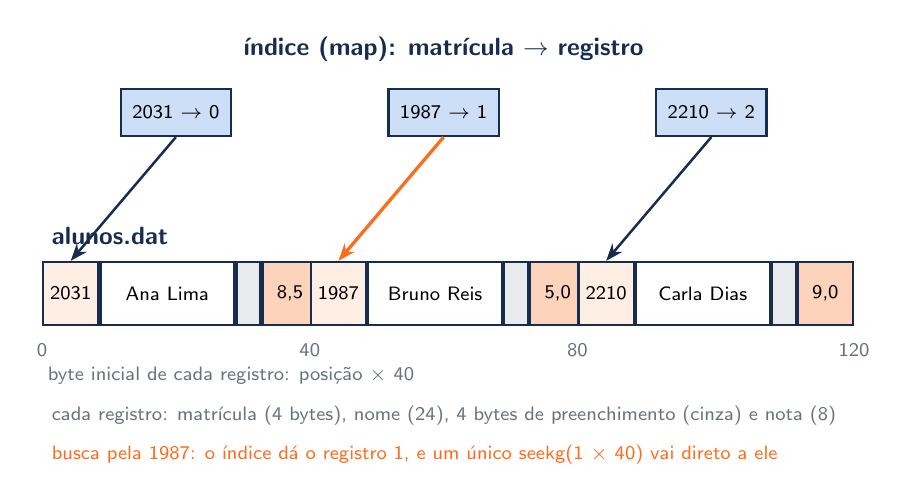
\begin{tikzpicture}
  \registro{r0}{0}{2031}{Ana Lima}{8,5}
  \registro{r1}{3.4}{1987}{Bruno Reis}{5,0}
  \registro{r2}{6.8}{2210}{Carla Dias}{9,0}
  \node[byte, below=1mm of r0m.south west, anchor=north] {0};
  \node[byte, below=1mm of r1m.south west, anchor=north] {40};
  \node[byte, below=1mm of r2m.south west, anchor=north] {80};
  \node[byte, below=1mm of r2v.south east, anchor=north] {120};
  \node[legenda, anchor=west] at (-0.05, -1.05)
    {byte inicial de cada registro: posição $\times$ 40};
  \node[rotulo, anchor=south west] at (0, 0.5) {alunos.dat};

  % índice em memória
  \node[rotulo] at (5.1, 3.1) {índice (map): matrícula $\rightarrow$ registro};
  \node[chaveidx] (i0) at (1.7, 2.3) {2031 $\rightarrow$ 0};
  \node[chaveidx] (i1) at (5.1, 2.3) {1987 $\rightarrow$ 1};
  \node[chaveidx] (i2) at (8.5, 2.3) {2210 $\rightarrow$ 2};
  \draw[seta] (i0.south) -- (r0m.north);
  \draw[seta, laranja, line width=1.2pt] (i1.south) -- (r1m.north);
  \draw[seta] (i2.south) -- (r2m.north);

  % legenda dos campos
  \node[legenda, align=left, anchor=west] at (0, -1.55)
    {cada registro: matrícula (4 bytes), nome (24), 4 bytes de preenchimento (cinza) e nota (8)};
  \node[legenda, text=laranja, align=left, anchor=west] at (0, -2.05)
    {busca pela 1987: o índice dá o registro 1, e um único seekg(1 $\times$ 40) vai direto a ele};
\end{tikzpicture}
\end{document}
